\documentclass[11pt,letterpaper]{article}
\usepackage{../acl2015}
\usepackage{times}
\usepackage{latexsym}
% \setlength\titlebox{7.5cm}    % Expanding the titlebox

%%% Custom additions %%%
\usepackage{url}
\usepackage[leqno, fleqn]{amsmath}
\usepackage{amssymb}
\usepackage{qtree}
\usepackage{graphicx}
\usepackage{booktabs}
\usepackage{multirow}
\usepackage{colortbl}
\usepackage{caption}
\usepackage{subcaption}
\usepackage{color}
\usepackage{xcolor}
\usepackage{tikz}
\usepackage{tikz-qtree}
\usepackage{ifthen}
\usepackage{framed}


\newcommand\todo[1]{\textcolor{blue}{\textbf{TODO:} #1}}
\newcommand\result[1]{\textcolor{red}{\textbf{RESULT NEEDED:} #1}}
\newcommand\question[1]{\textcolor{orange}{\textbf{OPEN QUESTION:} #1}}

\newcount\colveccount
\newcommand*\colvec[1]{
        \global\colveccount#1
        \begin{bmatrix}
        \colvecnext
}
\def\colvecnext#1{
        #1
        \global\advance\colveccount-1
        \ifnum\colveccount>0
                \\
                \expandafter\colvecnext
        \else
                \end{bmatrix}
        \fi
}

\newcommand{\nateq}{\equiv}
\newcommand{\natind}{\mathbin{\#}}
\newcommand{\natneg}{\mathbin{^{\wedge}}}
\newcommand{\natfor}{\sqsubset}
\newcommand{\natrev}{\sqsupset}
\newcommand{\natalt}{\mathbin{|}}
\newcommand{\natcov}{\mathbin{\smallsmile}}

\newcommand{\plneg}{\mathop{\textit{not}}}
\newcommand{\pland}{\mathbin{\textit{and}}}
\newcommand{\plor}{\mathbin{\textit{or}}}

\newcommand{\shift}{\textsc{shift}}
\newcommand{\reduce}{\textsc{reduce}}

% Strikeout
\newlength{\howlong}\newcommand{\strikeout}[1]{\settowidth{\howlong}{#1}#1\unitlength0.5ex%
\begin{picture}(0,0)\put(0,1){\line(-1,0){\howlong\divide\unitlength}}\end{picture}}

\newcommand{\True}{\texttt{T}}
\newcommand{\False}{\texttt{F}}
\usepackage{stmaryrd}
\newcommand{\sem}[1]{\ensuremath{\llbracket#1\rrbracket}}

\newcommand{\mynote}[1]{{\color{blue}#1}}
\newcommand{\tbchecked}[1]{{\color{red}#1}}

\usepackage{gb4e}
\noautomath
 
\def\ii#1{\textit{#1}}
\newcommand{\word}[1]{\emph{#1}}
\newcommand{\fulllabel}[2]{\b{#1}\newline\textsc{#2}}


%%%%%%%%%%%%%%%%%%%%%%%%%%%%%%%%%%%%%%%%%%%%%%%%%%%%%%%%%%%%%%%%%%%%%%
%%%%% Code to simulate natbib's citealt, which prints citations with
%%%%% no parentheses:

\makeatletter
\def\citealt{\def\citename##1{{\frenchspacing##1} }\@internalcitec}
\def\@citexc[#1]#2{\if@filesw\immediate\write\@auxout{\string\citation{#2}}\fi
  \def\@citea{}\@citealt{\@for\@citeb:=#2\do
    {\@citea\def\@citea{;\penalty\@m\ }\@ifundefined
       {b@\@citeb}{{\bf ?}\@warning
       {Citation `\@citeb' on page \thepage \space undefined}}%
{\csname b@\@citeb\endcsname}}}{#1}}
\def\@internalcitec{\@ifnextchar [{\@tempswatrue\@citexc}{\@tempswafalse\@citexc[]}}
\def\@citealt#1#2{{#1\if@tempswa, #2\fi}}
\makeatother

%%%%%%%%%%%%%%%%%%%%%%%%%%%%%%%%%%%%%%%%%%%%%%%%%%%%%%%%%%%%%%%%%%%%%

\title{Tree-structured neural networks revisited}

\author{
Samuel R.\ Bowman$^{1,2,5,}$\thanks{The first two authors contributed equally.} \\
\texttt{\small sbowman@stanford.edu} \\
\And
Jon Gauthier$^{2,3,5,*}$ \\
\texttt{\small jgauthie@stanford.edu} \\
\And
Abhinav Rastogi$^{4,5}$ \\
\texttt{\small arastogi@stanford.edu} \\
\AND
Raghav Gupta$^{6}$ \\
\texttt{\small rgupta93@stanford.edu} \\
\And
Christopher D.\ Manning$^{1,2,5,6}$\\
\texttt{\small manning@stanford.edu}\\
\And
Christopher Potts$^{1}$\\
\texttt{\small cgpotts@stanford.edu}
\AND\\[-3ex]
{$^{1}$Stanford Linguistics\quad
$^{2}$Stanford NLP Group\quad
$^{3}$Stanford Symbolic Systems}\\
{$^{4}$Stanford Electrical Engineering\quad
$^{5}$Stanford AI Lab\quad
$^{6}$Stanford Computer Science}
}

\date{}

\makeatletter
\newcommand{\@BIBLABEL}{\@emptybiblabel}
\newcommand{\@emptybiblabel}[1]{}
\definecolor{black}{rgb}{0,0,0}
\makeatother
\usepackage[breaklinks, colorlinks, linkcolor=black, urlcolor=black, citecolor=black, draft]{hyperref}

\def\t#1{#1}
\def\b#1{\t{\textbf{#1}}}
\def\colspaceS{2.25mm}
\def\colspaceM{4.0mm}
\def\colspaceL{4.25mm}

\begin{document}
\maketitle
\begin{abstract}
\begin{itemize}
\item TreeRNNs are great, don't work for big data.
\item We present the transition-based TreeRNN implementation -- makes efficient training possible, show that it helps relative to seq models.
\item Further, attention has proven powerful for extending sequence models. We introduce constit-by-constit attention, and find it to be effective here, too.
\end{itemize}
\end{abstract}

\todo{Anonymize.}

\section{Introduction}

\begin{figure}[t]
\begin{subfigure}[t]{0.9\columnwidth}
\vspace{14em}
\todo{[SB] Figure showing why trees can't be batched.}

\caption{\label{fig:batching:bad}Trees are hard to batch.}
\end{subfigure}

\vspace{2em}

\begin{subfigure}[t]{0.9\columnwidth}
\vspace{14em}
\todo{[SB] Figure showing why trees can't be batched.}

\caption{\label{fig:batching:good}Sequences are easy to batch.}
\end{subfigure}
\end{figure}

\begin{itemize}

\item Brief history of TreeRNNs
\begin{itemize}
\item Lx theory suggests should be better than comparable sequence models via compositionality \cite{Partee84,Janssen97}.
\item In practice, results mixed but positive. \citealt{tai2015improved} shows dramatic gains on sentiment analysis using tree-structured models over sequence models. \citealt{li2015tree} shows mixed results. Both of these evaluations are limited to small datasets with only hundreds or thousands of training examples.
\item Larger evaluations have been impossible due to issues of computational efficiency. One aim of this paper is to mitigate these issues to make larger-scale experiments possible.
\item Note, though, that while tree structure can be seen as a bias, simply adding more data within reason may not be enough to get a sequence model to learn without that bias \citealt{bowman2015trees}.
\end{itemize}

\item Speed issues
\begin{itemize}
\item Efficient batched computation is a crucial enabling technology in allowing NNs to be used on large datasets. Since NNs require large datasets to be able to model complex problems like language understanding, this is crucial in NLP.
\item Tree structured neural networks can't be batched. As the schematic in Figure~\ref{fig:batching:bad} indicates, different sentences are assigned different trees, and there is no straightforward way of aligning these trees to synchronize computation in the conventional style of implementation.
\item Our proposed model builds on ideas from transition-based parsing to build a model which implements the same computations as a tree-structured model, but which can be efficiently batched. See Figure~\ref{fig:batching:good}.

\end{itemize}

\item Attention issues
\begin{itemize}
\item The technique of soft attention has proven to be exceptionally effective as a way of training neural network models for tasks like translation \cite{bahdanau2014neural,luong-pham-manning:2015:EMNLP} and natural language inference \cite{rocktaschel2015reasoning}.
\item This paper proposes two complementary extensions of the idea of attention to tree-structured models:
\begin{itemize}
\item Constituent-by-constituent attention, in which each node in the tree of one sentence is given a soft alignment to some node or nodes in a second sentence.
\item The mTreeLSTM, which uses a third tree structured model to accumulate information about the alignment between two sentences into a single feature vector. This builds on the notion of a matching LSTM or mLSTM from \citealt{DBLP:journals/corr/WangJ15b}.
\end{itemize}
\end{itemize}
\end{itemize}

\section{The transition-based sentence model}

\subsection{Intuition: Transition-based parsing}

Our model is based on a formalism adapted from transition-based parsing (\todo{What's a good classic citation for this?}).

\todo{[SB, JG] Brief into to transition-based parsing.}

\subsection{The model}

Our model, which is shown in Figure~\ref{fig:model:0}, takes the form of a transition-based parser, but it is designed to produce sentence representations given parse structures, rather than producing parse structures as its output, leading to the following differences:
\begin{itemize}
\item The model takes a sequence of transitions (\shift s or \reduce s) as input, rather than incorporating a decision function which chooses which transition to perform at each step.
\item The intermediate representations in the parser, including the representations of the tree structures on the stack, are vectors of a fixed length.
\item The \reduce~operation, which combines two trees or tree nodes on the stack into a single larger tree, is represented using a parametric neural network layer function (in particular, a TreeLSTM layer, after \citealt{tai2015improved}).
\item The intermediate states of the stack and buffer during parsing are stored during training. This makes it possible to learn the parameters of the composition function and the input word representations that are fed into the buffer using backpropagation on an objective function that depends on the final sentence representation that emerges at the head of the stack.
\item A novel tracking LSTM component is added to improve the model's ability to efficiently track the context in which each step is being performed.
\end{itemize}



%!TEX root = hard_stack_paper/paper.tex


\begin{figure*}[t]

\begin{subfigure}[t]{\textwidth}
\centering
\scalebox{0.6}{
 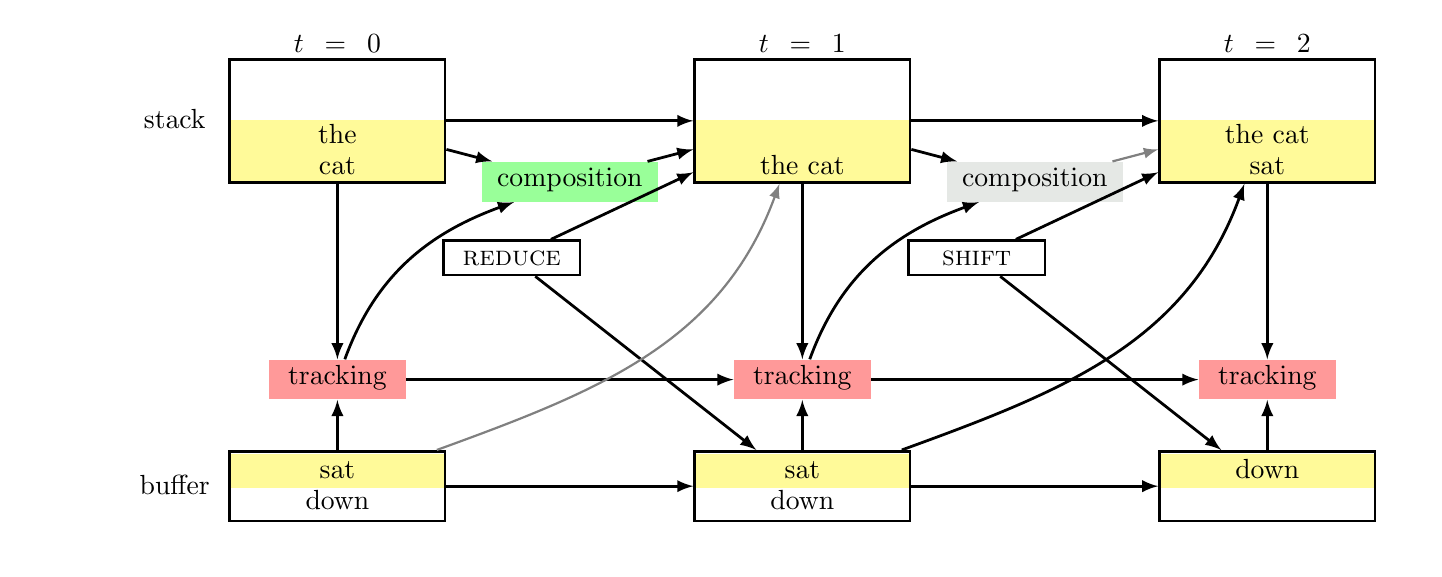
\begin{tikzpicture}
    \def\dx{21pt}
    \def\dy{11pt}
    \def\sy{13*\dy}
    \def\oxb{8*\dx}
    \def\by{1*\dy}
    \def\ox{0*\oxb}

    \tikzstyle{label}=[text width=35mm,align=center,text height=2mm]    
    \tikzstyle{word}=[text width=35mm,align=center,text height=2mm]    
    \tikzstyle{tracker}=[fill=red!40,text width=15mm,align=center,text height=2mm]
    \tikzstyle{softmax}=[fill=blue!40,text width=15mm,align=center,text height=2mm]
    \tikzstyle{comp}=[fill=green!40,text width=20mm,align=center,text height=2mm]
    \tikzstyle{compoff}=[fill=green!10!black!10,text width=20mm,align=center,text height=2mm]
    \tikzstyle{result}=[line width=1pt,draw=black,text width=15mm,align=center,text height=2mm]    
    \tikzstyle{sbox}=[line width=1pt,draw=black,text width=25mm,align=center,text height=13.3mm]
    \tikzstyle{bbox}=[line width=1pt,draw=black,text width=25mm,align=center,text height=6.5mm]
    \tikzstyle{focus1}=[fill=yellow!40,text width=25mm,align=center,text height=2mm]
    \tikzstyle{focus2}=[fill=yellow!40,text width=25mm,align=center,text height=5.5mm]

    \node[label]  (sl) at (\ox-0.35*\oxb+0*\dx,\by+0.5*\dy) {buffer};

    \node[label]  (1l) at (\ox+0*\dx,\sy+3*\dy) {$t=0$};

    \node[focus1] (0bb) at  (\ox+0*\dx,2*\dy) {};
    \node[word]  (0b3) at (\ox+0*\dx,\by-1*\dy) {};
    \node[word]  (0b2) at (\ox+0*\dx,\by+0*\dy) {down};
    \node[word]  (0b1) at (\ox+0*\dx,\by+1*\dy) {sat};
    \node[bbox] (0bb) at  (\ox+0*\dx,\by+0.5*\dy) {};
    
    \node[label]  (sl) at (\ox-0.35*\oxb+0*\dx,\sy+0.5*\dy) {stack};
    
    \node[focus2] (0sb) at  (\ox+0*\dx,\sy-0.5*\dy) {};
    \node[word]  (0s1) at (\ox+0*\dx,\sy-1*\dy) {cat};
    \node[word]  (0s2) at (\ox+0*\dx,\sy+0*\dy) {the};
    \node[word]  (0s3) at (\ox+0*\dx,\sy+1*\dy) {};
    \node[sbox] (0sb) at  (\ox+0*\dx,\sy+0.5*\dy) {};
    
    \node[comp] (0c) at  (\ox+0.5*\oxb,\sy-1.5*\dy) {composition};
    
    \node[tracker] (0t) at  (\ox+0*\dx,5*\dy) {tracking};
    % \node[softmax] (0sm) at  (\ox+3*\dx,7*\dy) {$\sigma$};
    \node[result] (0so) at  (\ox+3*\dx,9*\dy) {\reduce};
    
    \def\ox{1*\oxb}

    \node[label]  (1l) at (\ox+0*\dx,\sy+3*\dy) {$t=1$};

    \node[focus1] (1bb) at  (\ox+0*\dx,2*\dy) {};
    \node[word]  (1b3) at (\ox+0*\dx,\by-1*\dy) {};
    \node[word]  (1b2) at (\ox+0*\dx,\by+0*\dy) {down};
    \node[word]  (1b1) at (\ox+0*\dx,\by+1*\dy) {sat};
    \node[bbox] (1bb) at  (\ox+0*\dx,\by+0.5*\dy) {};
    
    \node[focus2] (1sb) at  (\ox+0*\dx,\sy-0.5*\dy) {};
    \node[word]  (1s1) at (\ox+0*\dx,\sy-1*\dy) {the cat};
    \node[word]  (1s2) at (\ox+0*\dx,\sy+0*\dy) {};
    \node[word]  (1s3) at (\ox+0*\dx,\sy+1*\dy) {};
    \node[sbox] (1sb) at  (\ox+0*\dx,\sy+0.5*\dy) {};
    
    \node[compoff] (1c) at  (\ox+0.5*\oxb,\sy-1.5*\dy) {composition};
    
    \node[tracker] (1t) at  (\ox+0*\dx,5*\dy) {tracking};
    % \node[softmax] (1sm) at  (\ox+3*\dx,7*\dy) {$\sigma$};
    \node[result] (1so) at  (\ox+3*\dx,9*\dy) {\shift};
     
    \def\ox{2*\oxb}

    \node[label]  (1l) at (\ox+0*\dx,\sy+3*\dy) {$t=2$};

    \node[focus1] (2bb) at  (\ox+0*\dx,2*\dy) {};
    \node[word]  (2b3) at (\ox+0*\dx,\by-1*\dy) {};
    \node[word]  (2b2) at (\ox+0*\dx,\by+0*\dy) {};
    \node[word]  (2b1) at (\ox+0*\dx,\by+1*\dy) {down};
    \node[bbox] (2bb) at  (\ox+0*\dx,\by+0.5*\dy) {};
    
    \node[focus2] (2sb) at  (\ox+0*\dx,\sy-0.5*\dy) {};
    \node[word]  (2s1) at (\ox+0*\dx,\sy-1*\dy) {sat};
    \node[word]  (2s2) at (\ox+0*\dx,\sy+0*\dy) {the cat};
    \node[word]  (2s3) at (\ox+0*\dx,\sy+1*\dy) {};
    \node[sbox] (2sb) at  (\ox+0*\dx,\sy+0.5*\dy) {};
   
    \node[tracker] (2t) at  (\ox+0*\dx,5*\dy) {tracking};

    
    \pgfsetarrowsend{latex}
    \tikzstyle{fwd} = [draw=black, line width=1pt]
    \tikzstyle{gated} = [draw=black!50, line width=0.8pt]

    \draw [fwd] (0sb) -- (0t);
    \draw [fwd] (0bb) -- (0t);
    \draw [fwd] (0sb) -- (0c);
    
    \draw [fwd] (0t) -- (1t);
    \draw [fwd] (0t) to[out=70,in=-160] (0c);
    \draw [fwd] (0sb) -- (1sb);
    \draw [fwd] (0bb) -- (1bb);
    \draw [fwd] (0so) -- (1sb);
    \draw [fwd] (0so) -- (1bb);
    \draw [gated] (0bb) to[out=20,in=-110] (1sb);
    \draw [fwd] (0c) -- (1sb);

    \draw [fwd] (1sb) -- (1t);
    \draw [fwd] (1bb) -- (1t);
    \draw [fwd] (1sb) -- (1c);
    
    \draw [fwd] (1t) -- (2t);
    \draw [fwd] (1t) to[out=70,in=-160] (1c);
    \draw [fwd] (1sb) -- (2sb);
    \draw [fwd] (1bb) -- (2bb);
    \draw [fwd] (1so) -- (2sb);
    \draw [fwd] (1so) -- (2bb);
    \draw [fwd] (1bb) to[out=20,in=-110] (2sb);
    \draw [gated] (1c) -- (2sb);

    \draw [fwd] (2sb) -- (2t);
    \draw [fwd] (2bb) -- (2t);


  \end{tikzpicture}}
  
 \caption{The model unrolled for two transitions on the input \word{the cat sat down}.}\label{fig:model:0}
  
\end{subfigure}\\\\\\
\begin{subfigure}[t]{\textwidth}
\centering
\scalebox{0.6}{
 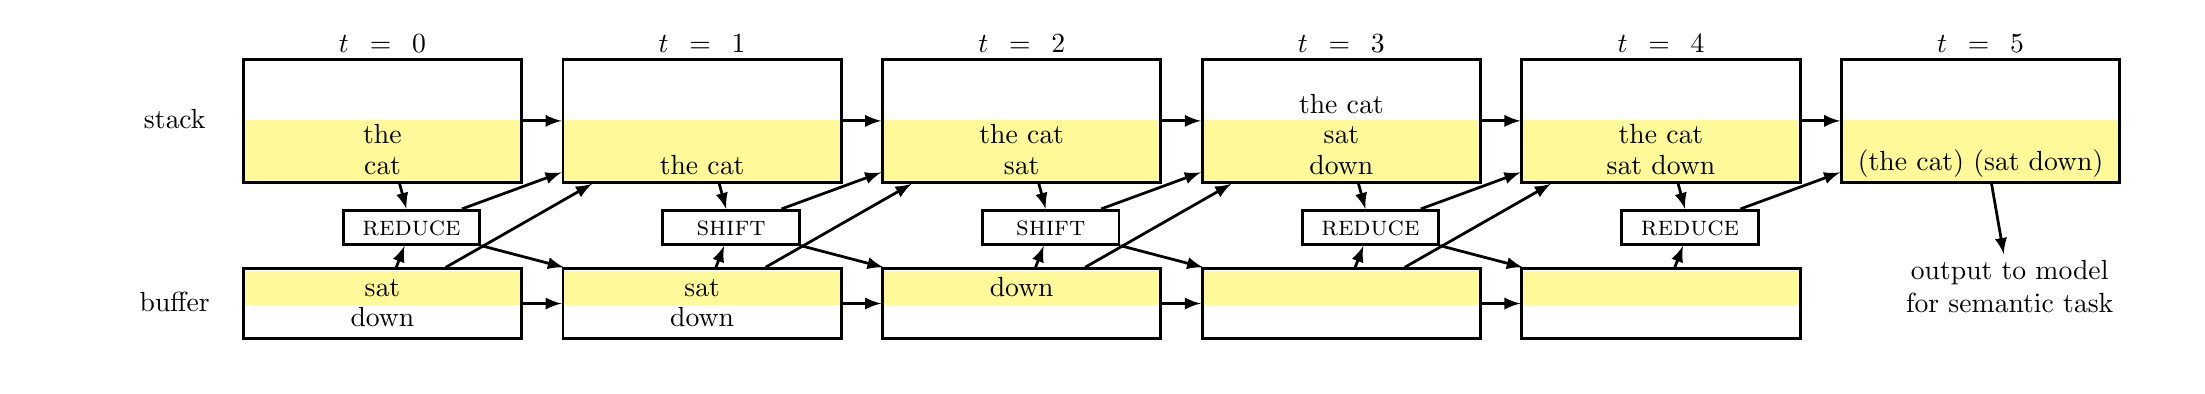
\begin{tikzpicture}
    \def\dx{21pt}
    \def\dy{11pt}
    \def\sy{7*\dy}
    \def\oxb{5.5*\dx}
    \def\by{1*\dy}
    \def\ox{0*\oxb}

    \tikzstyle{label}=[text width=35mm,align=center,text height=2mm]    
    \tikzstyle{word}=[text width=35mm,align=center,text height=2mm]    
    \tikzstyle{tracker}=[fill=red!40,text width=15mm,align=center,text height=2mm]
    \tikzstyle{softmax}=[text width=40mm,align=center,text height=2mm]
    \tikzstyle{comp}=[fill=green!40,text width=20mm,align=center,text height=2mm]
    \tikzstyle{result}=[line width=1pt,draw=black,text width=15mm,align=center,text height=2mm]    
    \tikzstyle{sbox}=[line width=1pt,draw=black,text width=33mm,align=center,text height=13.3mm]
    \tikzstyle{bbox}=[line width=1pt,draw=black,text width=33mm,align=center,text height=6.5mm]
    \tikzstyle{focus1}=[fill=yellow!40,text width=33mm,align=center,text height=2mm]
    \tikzstyle{focus2}=[fill=yellow!40,text width=33mm,align=center,text height=5.5mm]

    \def\ox{0*\oxb}
    
    \node[label]  (1l) at (\ox+0*\dx,\sy+3*\dy) {$t=0$};
    
    \node[label]  (sl) at (\ox-0.65*\oxb+0*\dx,\by+0.5*\dy) {buffer};
    
    \node[focus1] (1bb) at  (\ox+0*\dx,2*\dy) {};
    \node[word]  (1b3) at (\ox+0*\dx,\by-1*\dy) {};
    \node[word]  (1b2) at (\ox+0*\dx,\by+0*\dy) {down};
    \node[word]  (1b1) at (\ox+0*\dx,\by+1*\dy) {sat};
    \node[bbox] (1bb) at  (\ox+0*\dx,\by+0.5*\dy) {};
    
    \node[label]  (sl) at (\ox-0.65*\oxb+0*\dx,\sy+0.5*\dy) {stack};
    
    \node[focus2] (1sb) at  (\ox+0*\dx,\sy-0.5*\dy) {};
    \node[word]  (1s1) at (\ox+0*\dx,\sy-1*\dy) {cat};
    \node[word]  (1s2) at (\ox+0*\dx,\sy+0*\dy) {the};
    \node[word]  (1s3) at (\ox+0*\dx,\sy+1*\dy) {};
    \node[sbox] (1sb) at  (\ox+0*\dx,\sy+0.5*\dy) {};
    
    \node[result] (1so) at  (\ox+0.5*\dx,4*\dy) {\reduce};
              
    \def\ox{1*\oxb}
   
    \node[label]  (1l) at (\ox+0*\dx,\sy+3*\dy) {$t=1$};
    
    \node[focus1] (2bb) at  (\ox+0*\dx,2*\dy) {};
    \node[word]  (2b3) at (\ox+0*\dx,\by-1*\dy) {};
    \node[word]  (2b2) at (\ox+0*\dx,\by+0*\dy) {down};
    \node[word]  (2b1) at (\ox+0*\dx,\by+1*\dy) {sat};
    \node[bbox] (2bb) at  (\ox+0*\dx,\by+0.5*\dy) {};
    
    \node[focus2] (2sb) at  (\ox+0*\dx,\sy-0.5*\dy) {};
    \node[word]  (2s1) at (\ox+0*\dx,\sy-1*\dy) {the cat};
    \node[word]  (2s2) at (\ox+0*\dx,\sy+0*\dy) {};
    \node[word]  (2s3) at (\ox+0*\dx,\sy+1*\dy) {};
    \node[sbox] (2sb) at  (\ox+0*\dx,\sy+0.5*\dy) {};
    
    \node[result] (2so) at  (\ox+0.5*\dx,4*\dy) {\shift};
             
    \def\ox{2*\oxb}
    
    \node[label]  (1l) at (\ox+0*\dx,\sy+3*\dy) {$t=2$};
    
    \node[focus1] (3bb) at  (\ox+0*\dx,2*\dy) {};
    \node[word]  (3b3) at (\ox+0*\dx,\by-1*\dy) {};
    \node[word]  (3b2) at (\ox+0*\dx,\by+0*\dy) {};
    \node[word]  (3b1) at (\ox+0*\dx,\by+1*\dy) {down};
    \node[bbox] (3bb) at  (\ox+0*\dx,\by+0.5*\dy) {};
    
    \node[focus2] (3sb) at  (\ox+0*\dx,\sy-0.5*\dy) {};
    \node[word]  (3s1) at (\ox+0*\dx,\sy-1*\dy) {sat};
    \node[word]  (3s2) at (\ox+0*\dx,\sy+0*\dy) {the cat};
    \node[word]  (3s3) at (\ox+0*\dx,\sy+1*\dy) {};
    \node[sbox] (3sb) at  (\ox+0*\dx,\sy+0.5*\dy) {};
    
    \node[result] (3so) at  (\ox+0.5*\dx,4*\dy) {\shift};

    \def\ox{3*\oxb}
    
    \node[label]  (1l) at (\ox+0*\dx,\sy+3*\dy) {$t=3$};
        
    \node[focus1] (4bb) at  (\ox+0*\dx,2*\dy) {};
    \node[word]  (4b3) at (\ox+0*\dx,\by-1*\dy) {};
    \node[word]  (4b2) at (\ox+0*\dx,\by+0*\dy) {};
    \node[word]  (4b1) at (\ox+0*\dx,\by+1*\dy) {};
    \node[bbox] (4bb) at  (\ox+0*\dx,\by+0.5*\dy) {};
    
    \node[focus2] (4sb) at  (\ox+0*\dx,\sy-0.5*\dy) {};
    \node[word]  (4s1) at (\ox+0*\dx,\sy-1*\dy) {down};
    \node[word]  (4s2) at (\ox+0*\dx,\sy+0*\dy) {sat};
    \node[word]  (4s3) at (\ox+0*\dx,\sy+1*\dy) {the cat};
    \node[sbox] (4sb) at  (\ox+0*\dx,\sy+0.5*\dy) {};
    
    \node[result] (4so) at  (\ox+0.5*\dx,4*\dy) {\reduce};
                  
    \def\ox{4*\oxb}
    
    \node[label]  (1l) at (\ox+0*\dx,\sy+3*\dy) {$t=4$};
    
    \node[focus1] (5bb) at  (\ox+0*\dx,2*\dy) {};
    \node[word]  (5b3) at (\ox+0*\dx,\by-1*\dy) {};
    \node[word]  (5b2) at (\ox+0*\dx,\by+0*\dy) {};
    \node[word]  (5b1) at (\ox+0*\dx,\by+1*\dy) {};
    \node[bbox] (5bb) at  (\ox+0*\dx,\by+0.5*\dy) {};
    
    \node[focus2] (5sb) at  (\ox+0*\dx,\sy-0.5*\dy) {};
    \node[word]  (5s1) at (\ox+0*\dx,\sy-1*\dy) {sat down};
    \node[word]  (5s2) at (\ox+0*\dx,\sy+0*\dy) {the cat};
    \node[word]  (5s3) at (\ox+0*\dx,\sy+1*\dy) {};
    \node[sbox] (5sb) at  (\ox+0*\dx,\sy+0.5*\dy) {};
    
    \node[result] (5so) at  (\ox+0.5*\dx,4*\dy) {\reduce};
    
    \def\ox{5*\oxb}

    \node[label]  (1l) at (\ox+0*\dx,\sy+3*\dy) {$t=5$};

    \node[focus2] (6sb) at  (\ox+0*\dx,\sy-0.5*\dy) {};
    \node[word]  (6s1) at (\ox+0*\dx,\sy-1*\dy) {(the cat) (sat down)};
    \node[word]  (6s2) at (\ox+0*\dx,\sy+0*\dy) {};
    \node[word]  (6s3) at (\ox+0*\dx,\sy+1*\dy) {};
    \node[sbox] (6sb) at  (\ox+0*\dx,\sy+0.5*\dy) {};

    \node[softmax] (6sm) at  (\ox+0.5*\dx,2*\dy) {output to model for semantic task};
                   
    \pgfsetarrowsend{latex}
    \tikzstyle{fwd} = [draw=black, line width=1pt]

   \draw [fwd] (1sb) -- (1so);
   \draw [fwd] (1bb) -- (1so);

    \draw [fwd] (1sb) -- (2sb);
    \draw [fwd] (1bb) -- (2bb);
    \draw [fwd] (1so) -- (2sb);
    \draw [fwd] (1so) -- (2bb);
    \draw [fwd] (1bb) -- (2sb);

   \draw [fwd] (2sb) -- (2so);
   \draw [fwd] (2bb) -- (2so);

    \draw [fwd] (2sb) -- (3sb);
    \draw [fwd] (2bb) -- (3bb);
    \draw [fwd] (2so) -- (3sb);
    \draw [fwd] (2so) -- (3bb);
    \draw [fwd] (2bb) -- (3sb);

   \draw [fwd] (3sb) -- (3so);
   \draw [fwd] (3bb) -- (3so);

    \draw [fwd] (3sb) -- (4sb);
    \draw [fwd] (3bb) -- (4bb);
    \draw [fwd] (3so) -- (4sb);
    \draw [fwd] (3so) -- (4bb);
    \draw [fwd] (3bb) -- (4sb);

   \draw [fwd] (4sb) -- (4so);
   \draw [fwd] (4bb) -- (4so);

    \draw [fwd] (4sb) -- (5sb);
    \draw [fwd] (4bb) -- (5bb);
    \draw [fwd] (4so) -- (5sb);
    \draw [fwd] (4so) -- (5bb);
    \draw [fwd] (4bb) -- (5sb);

   \draw [fwd] (5sb) -- (5so);
   \draw [fwd] (5bb) -- (5so);

    \draw [fwd] (5sb) -- (6sb);
    \draw [fwd] (5so) -- (6sb);

   \draw [fwd] (6sb) -- (6sm);

  \end{tikzpicture}}
  
 \caption{The fully unrolled model for \word{the cat sat down} with some layers omitted for clarity.}\label{fig:model:1b}  
\end{subfigure}
\caption{\label{m1-views}Two views of the transition-based sentence model. In both views, the lower boxes represent the input buffer, and the upper boxes represent the stack. Yellow highlighting indicates which portions of these data structures are visible to the tracking LSTM and to the composition function. Thin gray arrows indicate connections which are blocked by a gating function, and so contribute no information. \todo{[SB] Clean up the arrangements of these figures now that we aren't reporting on Models 1/2.}}
\end{figure*}


\paragraph{Equivalence with existing models}
If we add no additional features, this model computes the same function as a plain TreeRNN. However, we expect it to be substantially faster than conventional TreeRNN implementations. Unlike a TreeRNN, the Model 0 computation graph is essentially static across examples, so examples of varying structures and lengths can be batched together and run on the same graph in a single step. This simply requires ensuring that the graph is run for enough timesteps to finish all of the sentences. This involves some wasted computation, since the composition function will be run $2N-1$ times (with the output of composition at non-\reduce~steps discarded), rather than $N-1$ times in a TreeRNN. However, this loss can be dramatically offset by the gains of batching, which stem from the ability to exploit highly optimized CPU and GPU libraries for batched matrix multiiplication. \todo{Update.}

\paragraph{The buffer and word representations}

We draw our word representations from the standard 300-dimensional vector package provided with GloVe \cite{pennington2014glove}. We do not update these vectors during training. Instead, we use a learned linear transformation to transform the representation of each input word $\vec{x}$ into a pair of vectors that can be used as inputs to a TreeLSTM composition function:

\begin{equation}
\colvec{2}
    {\vec{h}}
    {\vec{c}}
= W_{\text{wd}} \vec{x}
\end{equation}


\paragraph{The representations in the stack}

In our model, each row of the stack contains a pair of vectors $(h, c)$, which together represent some node in the parse tree of the sentence. Since the \shift~operation simply copies entries from the buffer onto the stack, this means that the word representations in the buffer also have two parts, $h$ and $c$. 

\paragraph{The composition function}

From \citealt{tai2015improved}.

The inputs to the composition function are the representations of the two words or phrases closest to the head of the, $(\vec{h}^1_s, \vec{c}^1_s)$ and $(\vec{h}^2_s, \vec{c}^2_s)$, which are treated as the two children of the tree node whose representation the composition function is constructing. Each vector is of the same dimension $D$.

\begin{gather}
\colvec{4}
    {\vec{i}}
    {\vec{f}_l}
    {\vec{f}_r}
    {\vec{o}}
= \sigma(
W_{\text{iffo}}
\colvec{3}
    {\vec{h}_s^1}
    {\vec{h}_s^2}
    {\vec{e}}
)
\\
\vec{g}
= \tanh(
W_{g}
\colvec{3}
    {\vec{h}_s^1}
    {\vec{h}_s^2}
    {\vec{e}}
)
\\
\vec{c} = \vec{f}_l * \vec{c}_s^2 + \vec{f}_r * \vec{c}_s^1 + \vec{i} * \vec{g}  
\\
\vec{h} = \vec{o} * \vec{c}
\end{gather}

$\vec{e}$ is an optional input argument which is either the empty vector $[]$ or a vector from an external source like the tracking LSTM (see below). $*$ denotes the elementwise product. Each vector-valued variable listed here is of dimension $D$. The values $(h, c)$ represent the local subtree, and both will be placed on the stack during a \reduce~operation.

\paragraph{The classifier}

This paper presents the transition-based sentence model within the context of \textit{natural language inference} (also known as \textit{recognizing textual entailment}), a sentence pair classification task. To classify a sentence pair, a feature vector is first constructed. This feature vector is based on the final representations of each of the two sentences---the representations that appear at the head of the stack for each sentence after the final transition. In particular, the $\vec{h}$ portions of these representations are used. The final feature vector consists of the concatenation of these two vectors, $\vec{x}_{\text{premise}}$ and $\vec{x}_{\text{hypothesis}}$, their difference, and their elementwise product:

\begin{equation}
\vec{x}_{classifier} = 
\colvec{4}
    {\vec{h}_{\text{premise}}}
    {\vec{h}_{\text{hypothesis}}}
    {\vec{h}_{\text{premise}} - \vec{h}_{\text{hypothesis}}}
    {\vec{h}_{\text{premise}} * \vec{h}_{\text{hypothesis}}}
\end{equation}

This feature vector is then passed to a series of two (\todo{Update}) ReLU neural network layers, then passed into a linear transformation, and then finally passed to a softmax layer, which yields a distribution among the three labels.

\subsection{Tracking left context with an auxiliary LSTM}

The tracking LSTM captures left context. \todo{Why?}

The tracking LSTM is a standard LSTM RNN. At each step it takes three vectors as inputs: the top element of the buffer $\vec{h}_b^1$, which would be moved in a \shift~operation, and the two two elements of the stack $\vec{h}_s^1$ and $\vec{h}_s^2$ which would be composed in a \reduce~operation. Its output hidden state at each step is used as the external input to the TreeLSTM composition function for that step.

\subsection{Implementing the transition-based sentence model}

\paragraph{The size of the stack}
The size of the stack should be $N$ for sentences of $N$ words, in case the first reduce merges the final two words. The size of the buffer should be $N$.

\paragraph{Converting parses to transition sequences}

For Models 0--3, all training data must be parsed in advance into an unlabeled binary constituency tree. In addition, Model 0 requires that  parses be available at test time as well. For both SST and SNLI we use the parses included with the corpus distributions whenever parses are needed. 

For model 0, training data can be prepared by linearizing the provided parse, then deleting left brackets and replacing right brackets with \reduce~instructions. That is demonstrated here with the example sentence \ii{the cat sat down}:

\begin{quote}\small
( ( the cat ) ( sat down ) )$\Rightarrow$\\
the cat \reduce~sat down \reduce~\reduce
\end{quote}

The input for models 1--4 is simply the word sequence from the parse, with the first two words moved into the stack. The syntactic supervision labels for models 1--3 are simply a binarized version of the Model 0 inputs, with the first two tokens (which are necessarily \shift~\shift) omitted: 

\begin{quote}\small
( ( the cat ) ( sat down ) )$\Rightarrow$ \\
stack: $\langle$the, cat$\rangle$\\
buffer: $\langle$sat, down$\rangle$\\
ops: \reduce~\shift~\shift~\reduce~\reduce
\end{quote}


\paragraph{Handling variable sentence lengths}

To efficiently implement batched computation, we must stipulate a fixed number of transitions (50) that the model can perform before producing an output. Sentences whose transition sequences are shorter than this length are padded, and sentences whose transition sequences are longer than this length are cropped. 

Padding, if done properly, should not impact the output of the model significantly:\footnote{The tracking LSTM can cause a slight dependence of the final representation on unrolling length. Because of this, we always train and test the model with a fixed unrolling length.} a model with the fixed parameters should produce the same representation for a 10-word sentence whether it is unrolled for 19 transitions (the minimum to avoid cropping) or 100.

Cropping necessarily discards information, but if done properly, it is nonetheless possible to learn good representations for cropped sentences. When a transition sequence is cropped, the number of removed \shift~transitions is tracked, and an equal number of word tokens is removed from the tail (left) end of the buffer. This makes it possible for a transition sequence to begin with a \reduce~transition, or to otherwise use a \reduce~transition on a stack that does not have two elements to reduce. In this instance, we simply feed the composition function one or more zero vectors, which represent nonexistent stack elements. If the composition learns to interpret these zero vectors properly, they can be taken to be unknown or incomplete nodes in an otherwise complete tree that is constructed according to the intended parse structure. \todo{[SB] Make a figure showing the results of cropping if there's room.}


\paragraph{Representing the stack in memory} Or, thin stack. 
\todo{[JG] Explain.}

\paragraph{Optimization and hyperparameters}

We used random search to tune \todo{[SB] List tuned hyperparameters.}

We trained each model for 250k steps, using a minibatch size of 64 for each step. We tracked each model's performance on the development set during training and saving parameters when this performance reached a new peak. We used early stopping, evaluating on the test set using the parameters that performed best on the development set.

\paragraph{Software infrastructure} We will make Theano code available.

\subsection{Related work: Transition-based parsing and neural networks.}

There has been a fairly long history of work on building neural-network based parsers that use the core operations and data structures from transition-based parsing \cite{henderson2004discriminative,emami2005neural,titov2010latent,buys2generative,chen2014,dyer-EtAl:2015:ACL-IJCNLP}. In addition, there has been recent work \cite{zhang2016top,dyer2016rnn} proposing models designed primarily for generative language modeling tasks that use these structures as well. To our knowledge, our model is the first to use these structures for the purpose of sentence interpretation, rather than parsing or generation.

\section{Attention over trees}

%!TEX root = gist.tex

\begin{figure*}[t]
\centering
\scalebox{0.8}{
 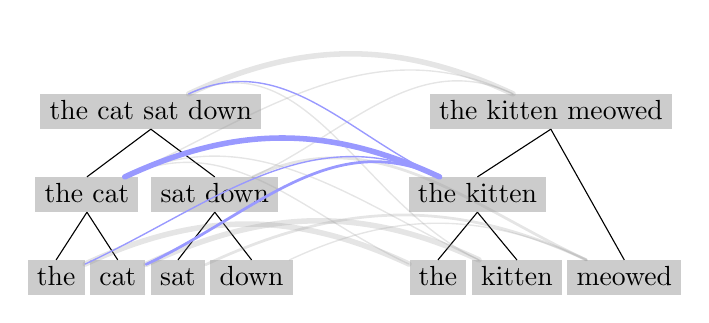
\begin{tikzpicture}
    \tikzstyle{word}=[fill=black!20,text height=2mm]    
    \tikzstyle{nonleaf}=[fill=black!20,text height=2mm]    

    \begin{scope}[shift={(0in,0in)}, frontier/.style={distance from root=60pt}]

    \Tree [.\node[nonleaf](1thecatsatdown){the cat sat down}; [.\node[nonleaf](1thecat){the cat}; \node[word](1the){the}; \node[word](1cat){cat}; ] [.\node[nonleaf](1satdown){sat down}; \node[word](1sat){sat}; \node[word](1down){down}; ] ]

    \end{scope}

    \begin{scope}[shift={(2in,0in)}, frontier/.style={distance from root=60pt}]

    \Tree [.\node[nonleaf](2thekittenmeowed){the kitten meowed}; [.\node[nonleaf](2thekitten){the kitten}; \node[word](2the){the}; \node[word](2kitten){kitten}; ] \node[word](2meowed){meowed}; ]

    \end{scope}
    
    \usetikzlibrary{arrows,scopes}

    \tikzstyle{attn} = [line width=1pt,draw=black!40,opacity=0.25,line cap=round]
    \tikzstyle{heavy} = [line width=2pt]
    \tikzstyle{light} = [line width=0.5pt]
    \tikzstyle{focus} = [draw=blue!40,opacity=1.0]

    \draw [attn,heavy] (1the) to[in=155,out=25] (2the);
    \draw [attn,light] (1thecat) to[in=155,out=25] (2the);

    \draw [attn,heavy] (1cat) to[in=155,out=25] (2kitten);
    \draw [attn,light] (1thecat) to[in=155,out=25] (2kitten);
    \draw [attn,light] (1thecatsatdown) to[in=155,out=25] (2kitten);

    \draw [attn,light] (1satdown) to[in=155,out=25] (2thekittenmeowed);
    \draw [attn,light] (1thecat) to[in=155,out=25] (2thekittenmeowed);
    \draw [attn,heavy] (1thecatsatdown) to[in=155,out=25] (2thekittenmeowed);

    \draw [attn] (1satdown) to[in=155,out=25] (2meowed);
    \draw [attn] (1sat) to[in=155,out=25] (2meowed);
    \draw [attn,light] (1down) to[in=155,out=25] (2meowed);

    \draw [attn,focus] (1cat) to[in=155,out=25,] (2thekitten);
    \draw [attn,heavy,focus] (1thecat) to[in=155,out=25] (2thekitten);
    \draw [attn,light,focus] (1the) to[in=155,out=25] (2thekitten);
    \draw [attn,light,focus] (1thecatsatdown) to[in=155,out=25] (2thekitten);

  \end{tikzpicture}}
  
 \caption{Soft alignments between the nodes of two trees, with alignments to ``the kitten'' highlighted in blue.}\label{fig:tree_attn}
\end{figure*}


\paragraph{Constituent-by-constituent attention}
We aim to build on the results of \citealt{rocktaschel2015reasoning} and \citealt{wang2015learning}, who find that neural soft attention models is an extremely effective technique for learning natural language inference. In particular, both papers use versions of word-by-word entailment, in which a latent alignment is learned from every word in the hypothesis to one or more words of the premise. We propose to borrow this basic idea, but to adapt it to a tree-structured setting, proposing \textit{constituent-by-constituent} attention. While these models do attention over a matrix $\mathbf{Y}$ of word-in-context representations from the premise encoder, we will perform attention instead over our own primary data structure, $\mathbf{Y}^{st}$, the matrix of vectors that have appeared at the top of the stack during premise encoding, which correspond one-to-one to the constituents in the tree structure representing the premise. Similarly, while the previous models perform one instance of soft attention conditioned on each word in the hypothesis, we perform one instance of soft attention conditioned on each stack top in the hypothesis encoder, representing the constituents of the hypothesis tree.

In our model, attention is performed at each step $t$ of the premise encoder. At step $t$, the query vector that drives attention will be $S^t_0$, the top of the stack. 

\todo{[AR, RG] Write up the attention equations that you use.}

\subsection{Accumulating the results of attention}

\paragraph{Accumulating results sequentially} (After Rocktäschel, Wang and Jiang)

\paragraph{Accumulating results using a second tree layer}

\section{Experiments}

\paragraph{The Stanford Natural Language Inference task} 
We evaluate our model on the Stanford Natural Language Inference task \cite{snli:emnlp2015}. 

550k/10k/10k split

We skip unlabeled examples.

\todo{[SB] Pull out an example from SNLI.}

We evaluate five models on the SNLI task. Each uses 150d hidden states: 
\begin{itemize}
\item A baseline LSTM model (similar to that of \citealt{snli:emnlp2015}) that uses the same classifier architecture as our models, but encodes sentences using a single layer LSTM RNN sequence model.
\item The unaugmented transition-based sentence model.
\item The transition-based sentence model with the tracking LSTM.
\item The transition-based sentence model with the tracking LSTM and sequence-based attention over premise states.
\item The transition-based sentence model with the tracking LSTM and tree-based attention over premise states.
\end{itemize}

\begin{table*}[t]
  \centering\small
  \begin{tabular}{lcccc} 
    \toprule
Model                   & Trained params.    &   Train  &   Test \\
\midrule
\multicolumn{4}{c}{Previous non-NN results}\\
\midrule
Lexicalized classifier \cite{snli:emnlp2015}
                        & --                 &   99.7   &   78.2      \\
\midrule
\multicolumn{4}{c}{Previous NN results without attention}\\
\midrule
100d LSTM encoders \cite{snli:emnlp2015}
                        & 221k               &   84.8   &   77.6      \\
1024d pretrained GRU encoders \cite{DBLP:journals/corr/VendrovKFU15}
                        & 15m                &   98.8   &   81.4       \\
300d Tree-based CNN encoders \cite{mou2015recognizing}
                        & 3.5m               &   83.4   &   82.1       \\
\todo{[SB] Import baselines from page}  
                        & ?                  &   ?      &   81?       \\
\midrule
\multicolumn{4}{c}{Previous NN results with attention}\\
\midrule
100d LSTM w/ word-by-word attention \cite{rocktaschel2015reasoning}
                        & 252k               &   85.3   &   83.5       \\
300d mLSTM word-by-word attention model \cite{DBLP:journals/corr/WangJ15b}
                        & 1.9m               &   92.0   &   86.1      \\
300d LSTMN with deep attention fusion \cite{cheng2016long} (1.4m params) 92.3    89.1

                        & 1.4m               &   92.3   &   89.1      \\
\midrule
\multicolumn{4}{c}{New results}\\
\midrule150d LSTM RNN           & ?                  &   ?      &   81?       \\
150d TB TreeLSTM    
                        & ?                  &   ?      &   82?       \\
150d TB TreeLSTM w/ tracking    
                        & ?                  &   ?      &   82?       \\
150d TB TreeLSTM w/ tracking, sequence-based attn.        
                        & ?                  &   ?      &   82?       \\
150d TB TreeLSTM w/ tracking, tree-based attn.            
                        & ?                  &   ?      &   \textbf{82?}\\
    \bottomrule
  \end{tabular}
  \protect\caption{\protect\label{tab:results}Results on SNLI 3-way inference classification. All reported figures are percent accuracy. \todo{Add seconds-per-step *if* we get a reasonably well-optimized model in time.}} 
\end{table*}

\paragraph{Results}

Table~\ref{tab:results} shows our results.

\subsection{Step time}

\todo{[JG,SB] Does anyone know of a better baseline TreeRNN implementation that we can use on Jagupard? We can use the CoreNLP SST model, but using a Java model as a baseline seems worrying unless we're guaranteed that it's competitively fast.}

Comparing model step time to the plain RNN of \citealt{li2015tree}. We use the small \citealt{pang2004sentimental} sentiment corpus that they use, and train with identical hyperparameters: ...

Evaluation metrics: Time per minibatch on a jag machine, with and without GPU access.

\section{Discussion}

\paragraph{Patterns in the examples that the tree model got right that the LSTM didn't}

\paragraph{Induced alignments}

\begin{figure}
\vspace{14em}
\caption{\label{fig:induced-alignment}The alignment induced between two sentences by \todo{some model.}. Compare with a similar alignment presented by \protect\citealt{DBLP:journals/corr/WangJ15b}.}
\end{figure}

\section{Conclusions and future work}

\begin{itemize}
\item It is possible to train a tree-structured model, without approximation, on large-scale language learning tasks.
\item Tree structure helps in large-scale language learning tasks. Not massively, but measurably.
\item The advantages of attention carry over to tree-structured models.
\item Future work: Encode the stack, after \citealt{dyer-EtAl:2015:ACL-IJCNLP}
\item Future work: Incorporate the parser
\item Future work: Latent parses
\end{itemize}

\subsubsection*{Acknowledgments}

(some of) the Tesla K40(s) used for this research was/were donated by the NVIDIA Corporation.

\bibliographystyle{../acl}
\bibliography{../MLSemantics} 

\end{document}
